\documentclass[aspectratio=169]{beamer}
\usepackage{mathtools,amsfonts}
\usepackage{tikz}
\usetikzlibrary{shapes.misc}
\usetikzlibrary{positioning}   % <-- nötig für "right=of box"
\usetikzlibrary{shapes.misc, positioning}

\title{Konvergenzbegriffe in der Wahrscheinlichkeitstheorie}
\subtitle{Warum schwache Konvergenz nicht genügt –\\
pfadweises Zusammenwachsen und praktische Beispiele}
\author{Oliver Dürr}
\date{\today}

\begin{document}
%----------------------------------------------------------
\begin{frame}[c,plain]
  \titlepage
\end{frame}

% ====== SLIDE 1 ==================================================
\begin{frame}{Der naive Zufallsbegriff – "Black Box“}
\centering
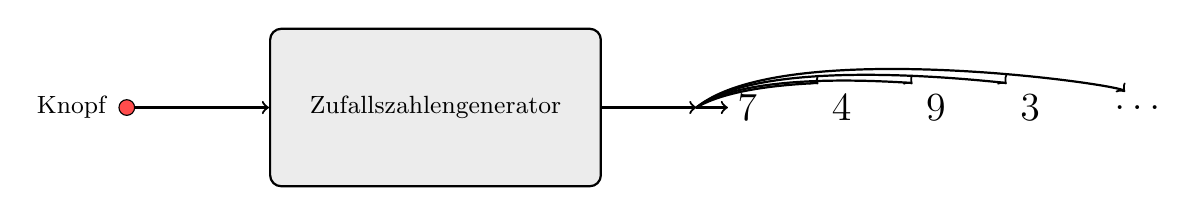
\begin{tikzpicture}[node distance=2.2cm, every node/.style={font=\small}]
      % Box
      \node[draw, thick, rounded corners, minimum width=4.2cm, minimum height=2cm,
                        fill=gray!15] (box) {Zufalls\-zahlengenerator};

      % Knopf­symbol
      \node[circle, draw, fill=red!70, inner sep=2pt, left=1.7cm of box] (btn) {};
      \node[left=1pt of btn] {\small Knopf};

      % Ein Pfeil von Knopf → Box
      \draw[->, thick] (btn) -- (box.west);

      % Output-Pfeil und viele Zahlen
      \draw[->, thick] (box.east) -- ++(1.2,0) coordinate (arrowend);
      \node[right=1.6cm of box] (n1) {\Large 7};
      \node[right=0.7cm of n1] (n2) {\Large 4};
      \node[right=0.7cm of n2] (n3) {\Large 9};
      \node[right=0.7cm of n3] (n4) {\Large 3};
      \node[right=0.7cm of n4] (dots) {\Large $\dots$};

      % Pfeile zu den Zahlen
      \draw[->, thick] (arrowend) -- (n1);
      \draw[->, thick, shorten >=2pt] (arrowend) .. controls +(0.5,0.3) and +(-0.3,0.3) .. (n2);
      \draw[->, thick, shorten >=2pt] (arrowend) .. controls +(0.7,0.5) and +(-0.3,0.3) .. (n3);
      \draw[->, thick, shorten >=2pt] (arrowend) .. controls +(0.9,0.7) and +(-0.3,0.3) .. (n4);
      \draw[->, thick, shorten >=2pt] (arrowend) .. controls +(1.1,0.9) and +(-0.3,0.3) .. (dots);
\end{tikzpicture}

\vspace{0.6em}
\begin{itemize}
  \item Jeder Knopfdruck liefert \textbf{eine Zahl}.  
  \item Viele Knopfdrücke $\;\Longrightarrow\;$ eine \textbf{empirische Verteilung}.  
  \item Die \emph{Zufallsquelle} (das $\omega$ aus $(\Omega,\mathcal F,P)$) bleibt unsichtbar.
\end{itemize}
\end{frame}

% ====== SLIDE 2 ==================================================
\begin{frame}{Konvergenz in Wahrscheinlichkeit}
\small
\textbf{Definition}  
\[
X_n \xrightarrow{\mathsf P} X
\quad\Longleftrightarrow\quad
\forall\varepsilon>0:\;
P\bigl(|X_n-X|>\varepsilon\bigr)\longrightarrow 0.
\]

\medskip
\textbf{Beispiel: empirische Verteilungsfunktion}  
Für i.i.d.\ $X_1,\dots,X_n$ mit Verteilungsfunktion $F$:
\[
F_n(x)=\tfrac1n\sum_{i=1}^n\mathbf1_{(X_i\le x)}
\quad\Longrightarrow\quad
F_n(x)\xrightarrow{\mathsf P}F(x)\quad(\text{f.\,j. fixes }x).
\]

\begin{block}{Intuition}
Der Schätzer $F_n(x)$ wird mit wachsendem $n$ \emph{wahrscheinlich} beliebig nah an die wahre Verteilungsfunktion $F(x)$ heranrücken.
\end{block}
\end{frame}

% ====== SLIDE 3 ==================================================
\begin{frame}{Zentraler Grenzwertsatz (i.i.d.-Version)}
\small
Seien $X_1,X_2,\dots$ i.i.d.\ mit $E[X_i]=\mu$ und $\operatorname{Var}(X_i)=\sigma^2<\infty$.

\[
\frac{\sqrt n\,(\bar X_n-\mu)}{\sigma}
\;\;\xrightarrow{\;d\;}\;\;
\mathcal N(0,1).
\]

\begin{itemize}
  \item $\bar X_n=\tfrac1n\sum_{i=1}^n X_i$  
  \item \emph{Konvergenz in Verteilung} – Zufallsstreuung bleibt erhalten.
\end{itemize}
\end{frame}

% ====== SLIDE 4 ==================================================
\begin{frame}{Gesetz der großen Zahlen – einfache Version}
\small
Für dieselben i.i.d.\ $X_i$:

\[
\bar X_n \xrightarrow{\mathsf P} \mu.
\]

\begin{block}{Lesart}
Mit wachsendem $n$ liegt der Stich­proben­mittelwert mit hoher Wahrscheinlichkeit beliebig nah am Erwartungswert~$\mu$.
\end{block}
\end{frame}

% ====== SLIDE 5 ==================================================
\begin{frame}{Gesetz der großen Zahlen – formale Version}
\small
\[
P\!\bigl(|\bar X_n-\mu|>\varepsilon\bigr)\;\longrightarrow_{n\to\infty}\;0,
\quad\forall\varepsilon>0.
\]

\medskip
\textbf{Kurzform $\;$vs.$\;$Ereignis‐Sprache}

\[
P\!\bigl(\underbrace{\{\omega:|\bar X_n(\omega)-\mu|>\varepsilon\}}_{\text{"zu weit weg"}}\bigr)\;\to 0.
\]

\begin{itemize}
  \item Die Differenz zu einer \textbf{Zufallsvariable} $Z\equiv\mu$ wird klein.  
  \item Schreibweise ohne $\omega$ ist nur Abkürzung – das Ereignis lebt in \(\Omega\).
\end{itemize}
\end{frame}

%----------------------------------------------------------
\begin{frame}{Intuition: Zufall $\to$ Verteilung (Black-Box-Bild)}
\centering
\begin{tikzpicture}[scale=1, every node/.style={font=\small}]
    % Zufallszahlengenerator (Box)
  \node[draw, thick, minimum width=4cm, minimum height=1.8cm, rounded corners, fill=gray!10] (box) {Zufalls\-zahlengenerator};

  % Output
  \node[right=of box] (output) {\Large $X(\omega)$};

  % Pfeile
  \draw[->, thick] (omega) -- (box);
  \draw[->, thick] (box) -- (output);

  % Knopf
  \node[draw, circle, fill=red!60, inner sep=2pt] (button) at (-2.2,0.8) {};
  \node[left=2pt of button] {Knopf};

  % Omega input
  %\node[draw, cloud, cloud puffs=12, cloud ignores aspect, minimum width=1cm, fill=blue!10] (omega) at (-2.5,-1.2) {$\omega$};
  %\draw[->, thick] (omega) -- (1.5,0.3);

  % Output arrows and numbers
  \draw[->, thick] (1.8,0) -- (3.2,0);
  \node at (3.9,0.4) {\Large 7};
  \node at (4.4,-0.1) {\Large 4};
  \node at (4.9,0.3) {\Large 9};
  \node at (5.4,-0.2) {\Large 3};
  \node at (5.8,0.1) {\Large $\dots$};

  % Histogram suggestion
  \draw[very thin] (3.2,-1.2) rectangle (5.8,-1.8);
  \draw[fill=gray!50] (3.3,-1.8) rectangle (3.4,-1.5);
  \draw[fill=gray!50] (3.5,-1.8) rectangle (3.6,-1.4);
  \draw[fill=gray!50] (3.7,-1.8) rectangle (3.8,-1.2);
  \draw[fill=gray!50] (3.9,-1.8) rectangle (4.0,-1.6);
  \draw[fill=gray!50] (4.1,-1.8) rectangle (4.2,-1.3);
  \node at (5.4,-1.5) {Histogramm};

\end{tikzpicture}

\vspace{1em}
\begin{itemize}
  \item Naive Sicht: \textit{Ein Knopfdruck $\to$ eine Zahl}.  
        Viele Knopfdrücke $\Rightarrow$ Häufigkeiten $\approx$ Verteilung.
  \item Unsichtbar bleibt der \textbf{Master-Zufall} $\omega\in\Omega$.  
        Eine Zufallsvariable ist nur die deterministische Abbildung $X(\omega)$.
\end{itemize}

\alert{Zentraler Punkt:}  
Ob zwei Variablen \emph{gemeinsam} konvergieren, hängt davon ab, ob sie denselben $\omega$ teilen.
\end{frame}


\begin{frame}{Intuition: Zufall $\to$ Verteilung (Black-Box-Bild)}
\centering
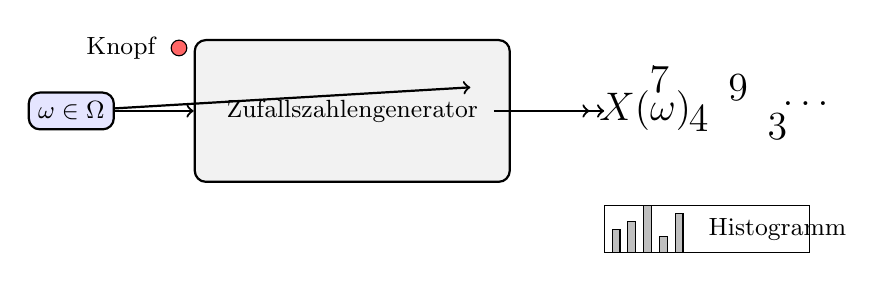
\begin{tikzpicture}[scale=1, every node/.style={font=\small}]
    % Zufallszahlengenerator (Box)
  \node[draw, thick, minimum width=4cm, minimum height=1.8cm, rounded corners, fill=gray!10] (box) {Zufalls\-zahlengenerator};

  % Omega-Input als abgerundete Box
  \node[draw, thick, rounded corners, fill=blue!10] (omega) [left=of box] {$\omega \in \Omega$};

  % Output
  \node[right=of box] (output) {\Large $X(\omega)$};

  % Pfeile
  \draw[->, thick] (omega) -- (box);
  \draw[->, thick] (box) -- (output);

  % Knopf
  \node[draw, circle, fill=red!60, inner sep=2pt] (button) at (-2.2,0.8) {};
  \node[left=2pt of button] {Knopf};

  % Omega input
  %\node[draw, cloud, cloud puffs=12, cloud ignores aspect, minimum width=1cm, fill=blue!10] (omega) at (-2.5,-1.2) {$\omega$};
  \draw[->, thick] (omega) -- (1.5,0.3);

  % Output arrows and numbers
  \draw[->, thick] (1.8,0) -- (3.2,0);
  \node at (3.9,0.4) {\Large 7};
  \node at (4.4,-0.1) {\Large 4};
  \node at (4.9,0.3) {\Large 9};
  \node at (5.4,-0.2) {\Large 3};
  \node at (5.8,0.1) {\Large $\dots$};

  % Histogram suggestion
  \draw[very thin] (3.2,-1.2) rectangle (5.8,-1.8);
  \draw[fill=gray!50] (3.3,-1.8) rectangle (3.4,-1.5);
  \draw[fill=gray!50] (3.5,-1.8) rectangle (3.6,-1.4);
  \draw[fill=gray!50] (3.7,-1.8) rectangle (3.8,-1.2);
  \draw[fill=gray!50] (3.9,-1.8) rectangle (4.0,-1.6);
  \draw[fill=gray!50] (4.1,-1.8) rectangle (4.2,-1.3);
  \node at (5.4,-1.5) {Histogramm};

\end{tikzpicture}

\vspace{1em}
\begin{itemize}
  \item Naive Sicht: \textit{Ein Knopfdruck $\to$ eine Zahl}.  
        Viele Knopfdrücke $\Rightarrow$ Häufigkeiten $\approx$ Verteilung.
  \item Unsichtbar bleibt der \textbf{Master-Zufall} $\omega\in\Omega$.  
        Eine Zufallsvariable ist nur die deterministische Abbildung $X(\omega)$.
\end{itemize}

\alert{Zentraler Punkt:}  
Ob zwei Variablen \emph{gemeinsam} konvergieren, hängt davon ab, ob sie denselben $\omega$ teilen.
\end{frame}

%----------------------------------------------------------
\begin{frame}{Zwei Konvergenzbegriffe – Definitionen}
\small
\textbf{Konvergenz in Verteilung (schwach)}

$X_n \xrightarrow{d} X 
\iff 
F_{X_n}(x)\to F_X(x)$ für alle Stetigkeitspunkte $x$.

\vspace{0.6em}
\textbf{Konvergenz in Wahrscheinlichkeit}

$X_n \xrightarrow{\mathsf P} X
\iff
\forall\varepsilon>0:\;
P(|X_n-X|>\varepsilon)\to0$.

\vspace{0.6em}
\textbf{Hierarchie}\; $\text{a.s.}\;\Rightarrow\;\mathsf P\;\Rightarrow\;d$

\begin{block}{Merke}
$\mathsf P$ vergleicht Pfade auf demselben $\omega$;  
$d$ vergleicht bloß Randverteilungen.
\end{block}
\end{frame}

%----------------------------------------------------------
\begin{frame}{Beispiel 1 – Empirische Verteilungsfunktion}
\small
$X_1,\dots,X_n$ i.i.d., Verteilungsfunktion $F$.  
$F_n(x)=\tfrac1n\sum_{i=1}^n\mathbf1_{(X_i\le x)}$.

$F_n(x)\xrightarrow{\mathsf P}F(x)$ für jedes feste $x$.

\vspace{0.4em}
Stärkere Glivenko–Cantelli-Aussage:  
$\sup_x|F_n(x)-F(x)|\xrightarrow{a.s.}0$.
\end{frame}

%----------------------------------------------------------
\begin{frame}{Beispiel 2 – Zentraler Grenzwertsatz}
\small
$(X_i)$ i.i.d., $E[X_i]=\mu$, $\operatorname{Var}(X_i)=\sigma^2$.

\[
\frac{\sqrt n\,(\bar X_n-\mu)}{\sigma}
\;\xrightarrow{d}\;
\mathcal N(0,1).
\]

Schwach $\Rightarrow$ Zufalls­struktur (Varianz 1) bleibt.
\end{frame}

%----------------------------------------------------------
\begin{frame}{LLN – einfache Version}
\small
\[
\bar X_n\;=\;\tfrac1n\sum_{i=1}^n X_i
\;\xrightarrow{\mathsf P}\;\mu.
\]

Pfaddeutung: Für fast jedes $\omega$ liegt $\bar X_n$ irgendwann $\varepsilon$-nah an $\mu$.
\end{frame}

%----------------------------------------------------------
\begin{frame}{LLN – formale Version}
\small
\[
P(|\bar X_n-\mu|>\varepsilon)\to0
\quad(\forall\varepsilon>0).
\]

Kurzform für  
$P\bigl\{\omega:|\bar X_n(\omega)-\mu|>\varepsilon\bigr\}\to0$.
\end{frame}

%----------------------------------------------------------
\begin{frame}{Kopplung vieler MCMC-Ketten}
\small
Quadratisches Potential $V(k)=k^2$, gemeinsamer RNG-Strom.  
Startwerte verschieden $\to$ Meeting‐Zeit $\tau_{\max}$.

\[
\forall i,j:\;
|X_t^{(i)}-X_t^{(j)}|\xrightarrow{\mathsf P}0
\quad\Longrightarrow\quad
X_t^{(i)}\xrightarrow{\mathsf P}Z,\;Z\sim\pi(k)\propto e^{-k^{2}}.
\]
\end{frame}

%----------------------------------------------------------
\begin{frame}{Zwei RNG-Streams – Seed-Effekt}
\small
\textbf{Unterschiedliche Seeds}

$X_n,Y_n$ Uniform(0,1).  
\[
P(|X_n-Y_n|>\varepsilon)\not\to0
\quad\Rightarrow\quad
X_n\not\xrightarrow{\mathsf P}Y_n.
\]

\textbf{Gemeinsamer Seed}

$X_n=Y_n$ $\forall n$
$\;\Rightarrow\;$ sofort $X_n\xrightarrow{\mathsf P}Y_n$.

Gleiche Randverteilungen $\neq$ Pfadnähe.
\end{frame}

%----------------------------------------------------------
\begin{frame}{Take-aways}
\begin{itemize}
  \item Schwache Konvergenz: nur Randverteilungen.  
  \item Konvergenz in Wahrscheinlichkeit: Pfade auf gleichem $\omega$.  
  \item Kopplungstricks zeigen den Unterschied praktisch (MCMC, Seeds).  
  \item Burn-in: notwendig, aber unabhängig von Pfadverschmelzung.
\end{itemize}
\end{frame}

%----------------------------------------------------------
\end{document}